\section{Data Memory}
\subsubsection{Overview}
In computer architecture, data memory is used to store data that is read from or written to by the processor. Data memory is typically implemented using an array of memory cells, each capable of holding a fixed amount of data, such as a byte or word. Key operations associated with data memory include:

\begin{itemize}
\item \textbf{Read Operation:} Retrieving data from a specific memory address.

\item \textbf{Write Operation:} Storing data at a specific memory address.

\item \textbf{Addressing:} Using an address to specify the location of data within the memory.
 \end{itemize}

 
\begin{figure}[H]
    \centering
    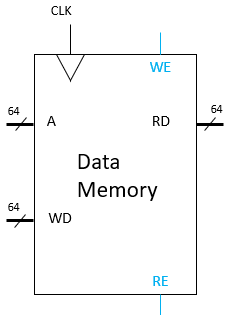
\includegraphics[width=0.3\linewidth]{Image/Data Memory.png}
    \caption{Data Memory}
    \label{fig:enter-label}
\end{figure}

\subsubsection{Implementation}
\textbf{Parameterization:}
\begin{itemize}
\item \textbf{Data Width:} The width of the data bus, which determines how much data can be read from or written to the memory in one operation. In the provided code, this is set to 64 bits.

\item \textbf{Address Width:} The width of the address bus, which determines the number of addressable memory locations. Here, it's set to 64 bits.
\end{itemize}
\textbf{Input/Output Interfaces:}
\begin{itemize}
\item \textbf{clk (input):} Clock signal to synchronize operations.
\item \textbf{memWriteEnable (input):} Control signal to enable writing to memory.
\item \textbf{memReadEnable (input):} Control signal to enable reading from memory.
\item \textbf{address (input):} 64-bit address bus specifying the memory location for read/write operations.
\item \textbf{writeData (input):} 64-bit data bus carrying the data to be written to memory.
\item \textbf{readData (output):} 64-bit data bus outputting the data read from memory.
\end{itemize}

\textbf{Memory Array:}

\begin{itemize}
\item The memory array is 128 bytes, organized as an array of 8-bit registers.
\end{itemize}

\textbf{Read and Write Operations:}

\begin{itemize}
\item Write operation should be synchronous with the clock signal.
\item Read operation should be combinational based on the control signal.
\item Data should be written and read in chunks of 64 bits, spread across 8 consecutive memory locations.
\end{itemize}

\textbf{Initialization:\textbf}
\begin{itemize}
\item The memory array should be initialized to zero during simulation.
\end{itemize}